\begin{tikzpicture}[scale = 0.13, show background rectangle]
\scriptsize
%\node[anchor=south west,inner sep=0] (image) at (0,0) {\includegraphics[width=0.8\textwidth]{110121_1431.png}};

% Board Außenmaße
%\draw[style = thick] (0,0) rectangle (68.6,50);

% Definition global
\tikzmath{
\bw = 0.5;
\w = \bw;
\mop = 0.9;
\op = \mop;
};

%%%%%%%
\node[anchor=north east,inner sep=0] (image) at (22,30) {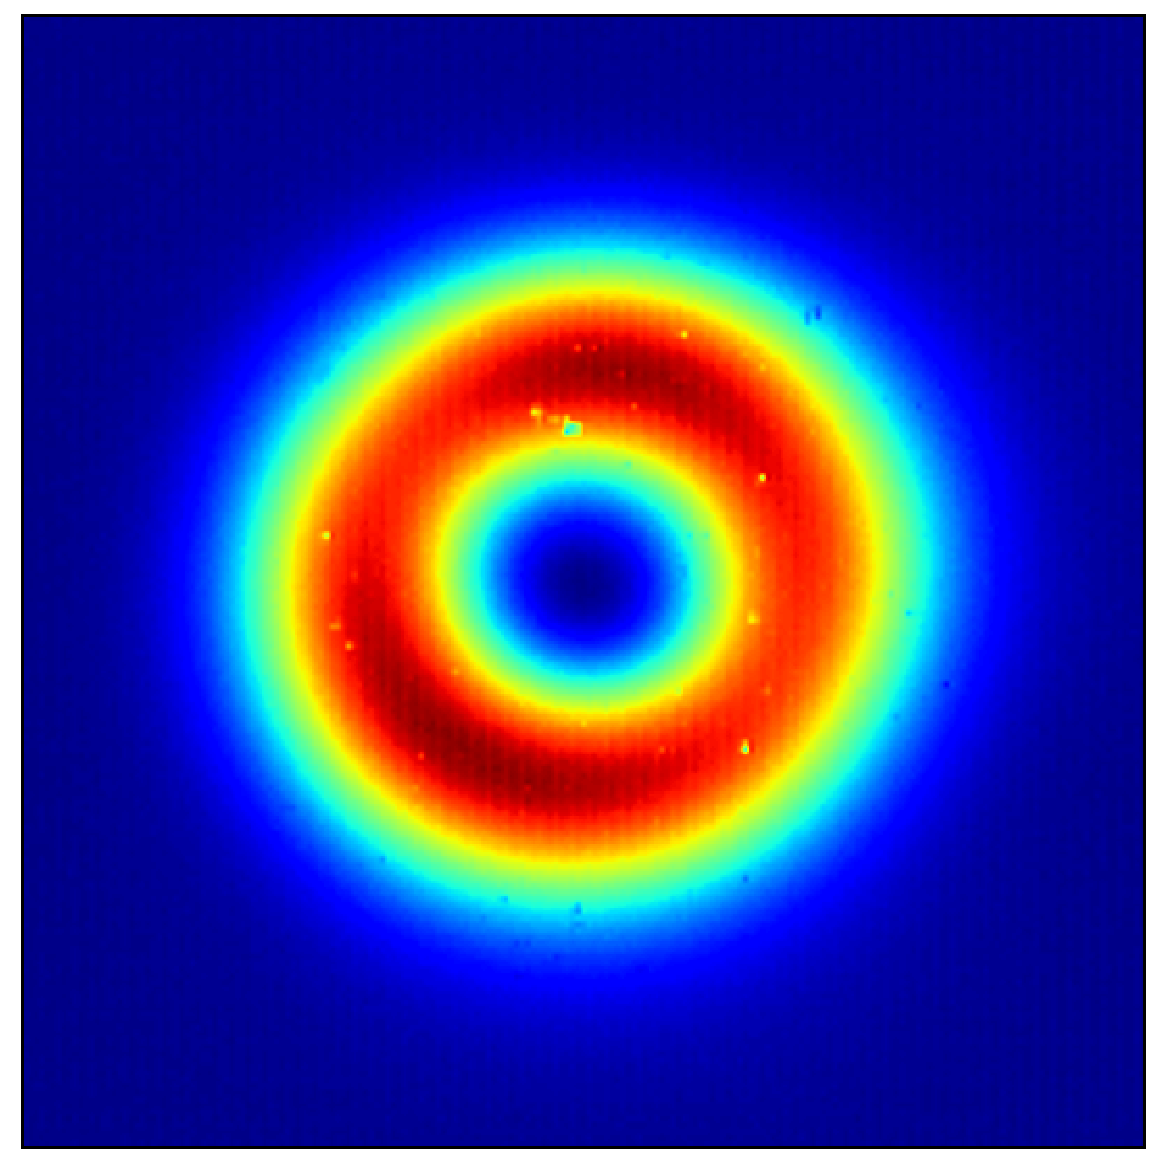
\includegraphics[width=0.2\textwidth]{graphics/Focalplane.pdf}};

\coordinate (focus) at (40, 38.5);
\coordinate (arrowstart) at (21.6,29.55);
\coordinate (corner) at (40,35);
\coordinate (textfocal) at (41,32);

\node[text width=22] at (textfocal){Focal Plane};
\draw[style=very thick, -Stealth] (arrowstart) -- (corner) -- (focus);

%%%%%%%
%reimaged focal plane
%%%%%%%
\coordinate (chambertr) at (54.2, 20.8);
\coordinate (textreimagfp) at (54, 24);
\draw[Stealth-] (chambertr) -- + (-2,2);
\tiny
\node[text width=50] at (textreimagfp){Relayed \\ Focal \\ Plane};
\scriptsize


%%%%%%%
%axes and gravitation
%%%%%%%

%\coordinate (origin) at (30,8.5);
%\coordinate (ordinate) at (30,13.5);
%\node at (28.5,13.5){\scriptsize{$z$}};
%\coordinate (abscissa) at (35,8.5);
%\node at (35,7){\scriptsize{$x$}};

\coordinate (gravity) at (60, 17);
\tiny
\node at (60,18){Gravity};
\scriptsize

\draw[-Stealth] (gravity) -- + (0,-3);

\coordinate (vacpointer) at (36,10);
\coordinate (textvac) at (32,10);
\node[text width=40] at (textvac){Vacuum \\ Chamber};

\draw[-Stealth] (vacpointer) -- + (9,2);

%\draw[->] (origin) -- (abscissa);
%\draw[->] (origin) -- (ordinate);



%%%%%%% Wesentliche Optiken
	\coordinate (Beamstart) at (5, 40);
		%\node at (4,43){AK};
	\coordinate (lam1) at (10, 40);
		\node at (10,44){$\lambda$/2};
	\coordinate (PST) at (17, 40);
		\node at (17,44){PBS};
	\coordinate (PO) at (23, 40);
	\coordinate (POL) at (23, 43);
	\coordinate (PD) at (23, 45);
		
		
	\coordinate (lam2) at (25, 40);
		%\node at (25,43){$\lambda$/2};
	\coordinate (lam3) at (30, 40);
		\node at (30,44){$\lambda$/4};
	\coordinate (L1) at (35, 40);
		\node at (35,44){L1};
	\coordinate (CR) at (39.5, 40);
		\node at (39.2,44){CR};
	\coordinate (L2) at (45, 40);
		\node at (45,44){L2};
	\coordinate (L3) at (50, 40);
		\node at (50,44){L3};
	\coordinate (NPST) at (55, 40);
		\node at (60,40){BS};
	\coordinate (Cam) at (55, 45);
	\coordinate (L4) at (55, 36);
		\node at (60,36){L4};
	\coordinate (L5) at (55, 33);
		\node at (60,33){L5};	
	\coordinate (chamber) at (55, 20);
		
	%%% Sonstiges
	\coordinate (fiberend) at (1, 36);	
	\coordinate (End) at (55, 7);
	
%%% Detection light
\coordinate (C1) at (55+0.5, 7);
\coordinate (C2) at (55-0.5, 7);
\coordinate (D1) at (55+0.5, 45);
\coordinate (D2) at (55-0.5, 45);

\fill[color = red, opacity = 0.5] (C1) -- (D1) -- (D2) -- (C2) -- cycle;

%%% blue beam:
\beamstart{Beamstart}{lam1}{\w};
\pickoff{PO}{PD}{2.54}{\w};
\avoidcrossedbeam;
\beam{POL}{90}{\w};
\photodiode{PD}{-90}{Beamstart};
\node at (23,47){PD};
\avoidcrossedbeam;
\beam{L1}{0}{\w};
\beam{L2}{180}{\w};
\avoidcrossedbeam;
\beam{L3}{0}{\w};
\avoidcrossedbeam;
\mirror{NPST}{L4}{0.}{0.};
\beam{L4}{90}{\w};
\avoidcrossedbeam;
\beam{L5}{-90}{\w};
\beam{End}{90}{\w};

%CDT beam
\coordinate (A1) at (42, 20+0.2);
\coordinate (A2) at (42, 20-0.2);
\coordinate (A3) at (68, 20+0.2);
\coordinate (A4) at (68, 20-0.2);
\fill[color = red, opacity = 1.] (A1) -- (A2) -- (A4) -- (A3) -- cycle;
\node[text width=60] at (38,20){Crossed \\ Dipole Trap};

%%%%%%%%%%%
% Drawing optics
%%%%%%%%%%%
\fibercollimator{Beamstart}{lam1}{fiberend}{0}{\w};
\plate{lam1}{\angB}{1.5};
\cube{PST}{\angB-45}{2.54};
\pickoffdraw{PO}{PD}{2.54}{\w};
\lensdraw{POL}{90}{2.54}{\w};
\plate{lam3}{\angB}{1.5};
\lensdraw{L1}{0}{5.08}{\w};
\platethick{CR}{0}{2.54}{1.28};
\lensdraw{L2}{180}{5.08}{\w};
\lensdraw{L3}{0}{5.08}{\w};
\cube{NPST}{45}{2.54};
\lensdraw{L4}{90}{5.08}{\w};
\lensdraw{L5}{-90}{5.08}{\w};
\CCD{Cam}{-90};
\node at (55,47.25){CCD};

%%%%%%%%%%%%
% Chamber
%%%%%%%%%%%%
\tikzmath{
\R = 12;
\r = 10;
\d1 = 5;
\d2 = 3;
\a1 = asin(\d1/(2*\r));
\a2 = asin(\d2/(2*\r));
\d0 = \R - \r;
\Rh = \R * cos(\a1);
};

\path (chamber) + (90:\Rh) coordinate (A);
\draw[] (A) -- ++ (0:\d1/2) -- ++ (-90:\d0) arc (90-\a1:45+\a2:\r) -- ++ (45:\d0) -- ++ (-45:\d2) -- ++ (-135:\d02) arc (45-\a2: \a1: \r) -- ++ (0:\d0) -- ++ (-90:\d1) -- ++ (180:\d0) arc (-\a1: -45+\a2: \r) -- ++ (-45:\d0) --++ (-135:\d2) --++ (135:\d0) arc(-45-\a2:-90+\a1:\r) --++ (-90:\d0) --++(180:\d1) --++ (90:\d0) arc (-90-\a1: -135+\a2:\r) --++ (-135:\d0) --++ (135:\d2) --++(45:\d0) arc (-135-\a2:-180+\a1:\r) --++ (180:\d01) --++ (90:\d1) --++ (0:\d0) arc(180-\a1:135+\a2:\r) --++ (135:\d02) --++ (45:\d2) --++ (-45:\d0) arc(135-\a2:90+\a1:\r) --++ (90:\d0) --cycle;  

\end{tikzpicture}